\documentclass[a4paper]{article}

%science unit
\usepackage{siunitx}

%image insertion
\usepackage{graphicx} %image settings
\DeclareGraphicsExtensions{.pdf,.png,.jpg, .gif}

%math
\usepackage{amsmath} %math
%\usepackage{cmbright} %math font

%font
\usepackage{kotex}
\usepackage{fontspec}
\ifx가가
\setmainhangulfont[Ligatures=TeX,
BoldFont={KoPubBatang Medium}]{KoPubBatang Light}
\setsanshangulfont[Ligatures=TeX,
BoldFont={KoPubDotum Medium}]{KoPubDotum Light}
\setmainhanjafont[Ligatures=TeX,
BoldFont={KoPubBatang Medium}]{KoPubBatang Light}
\setsanshanjafont[Ligatures=TeX,
BoldFont={KoPubDotum Medium}]{KoPubDotum Light}
\xetexkofontregime[puncts=prevfont, colons=prevfont, cjksymbols=hangul]{latin}
\fi

%줄간격
\usepackage{setspace}
\usepackage{indentfirst}
\setstretch{1.3}
\everydisplay{\setstretch{1.2}}

%subfigure
\usepackage{subfigure}

\pagestyle{plain}
\title{물리 실험보고서 2}
\author{이한빈, 의예과 2016-XXXXX}

\begin{document}


\numberwithin{equation}{section}
\maketitle

\section{Introduction}


	축전기는 전하를 저장하는 장치로 전압이 가해졌을 때 전압에 비례하는 양의 전하를 축적한다.
		\begin{equation} \label{eq:qcv}
			Q=CV
		\end{equation}

	(\ref{eq:qcv})에 쓰인 비례상수 C는 축전기의 기하학적 모양과 유전체의 종류에 의존한다. 본 실험에 쓰여진 평행판 축전기의 경우 극판의 면적이 $A$, 극판의 간격이 $d$일 때 다음으로 주어진다.
		\begin{equation} \label{eq:ppl}
			C=\epsilon \frac{A}{d} \quad (단, \: \epsilon는 \: 극판 \: 사이의  \: 유전상수)
		\end{equation}

	축전기의 모습을 그림으로 나타내면 다음과 같다.
		\begin{figure}[h]
			\centering
				\subfigure[Parallel Plate Capacitor]{
				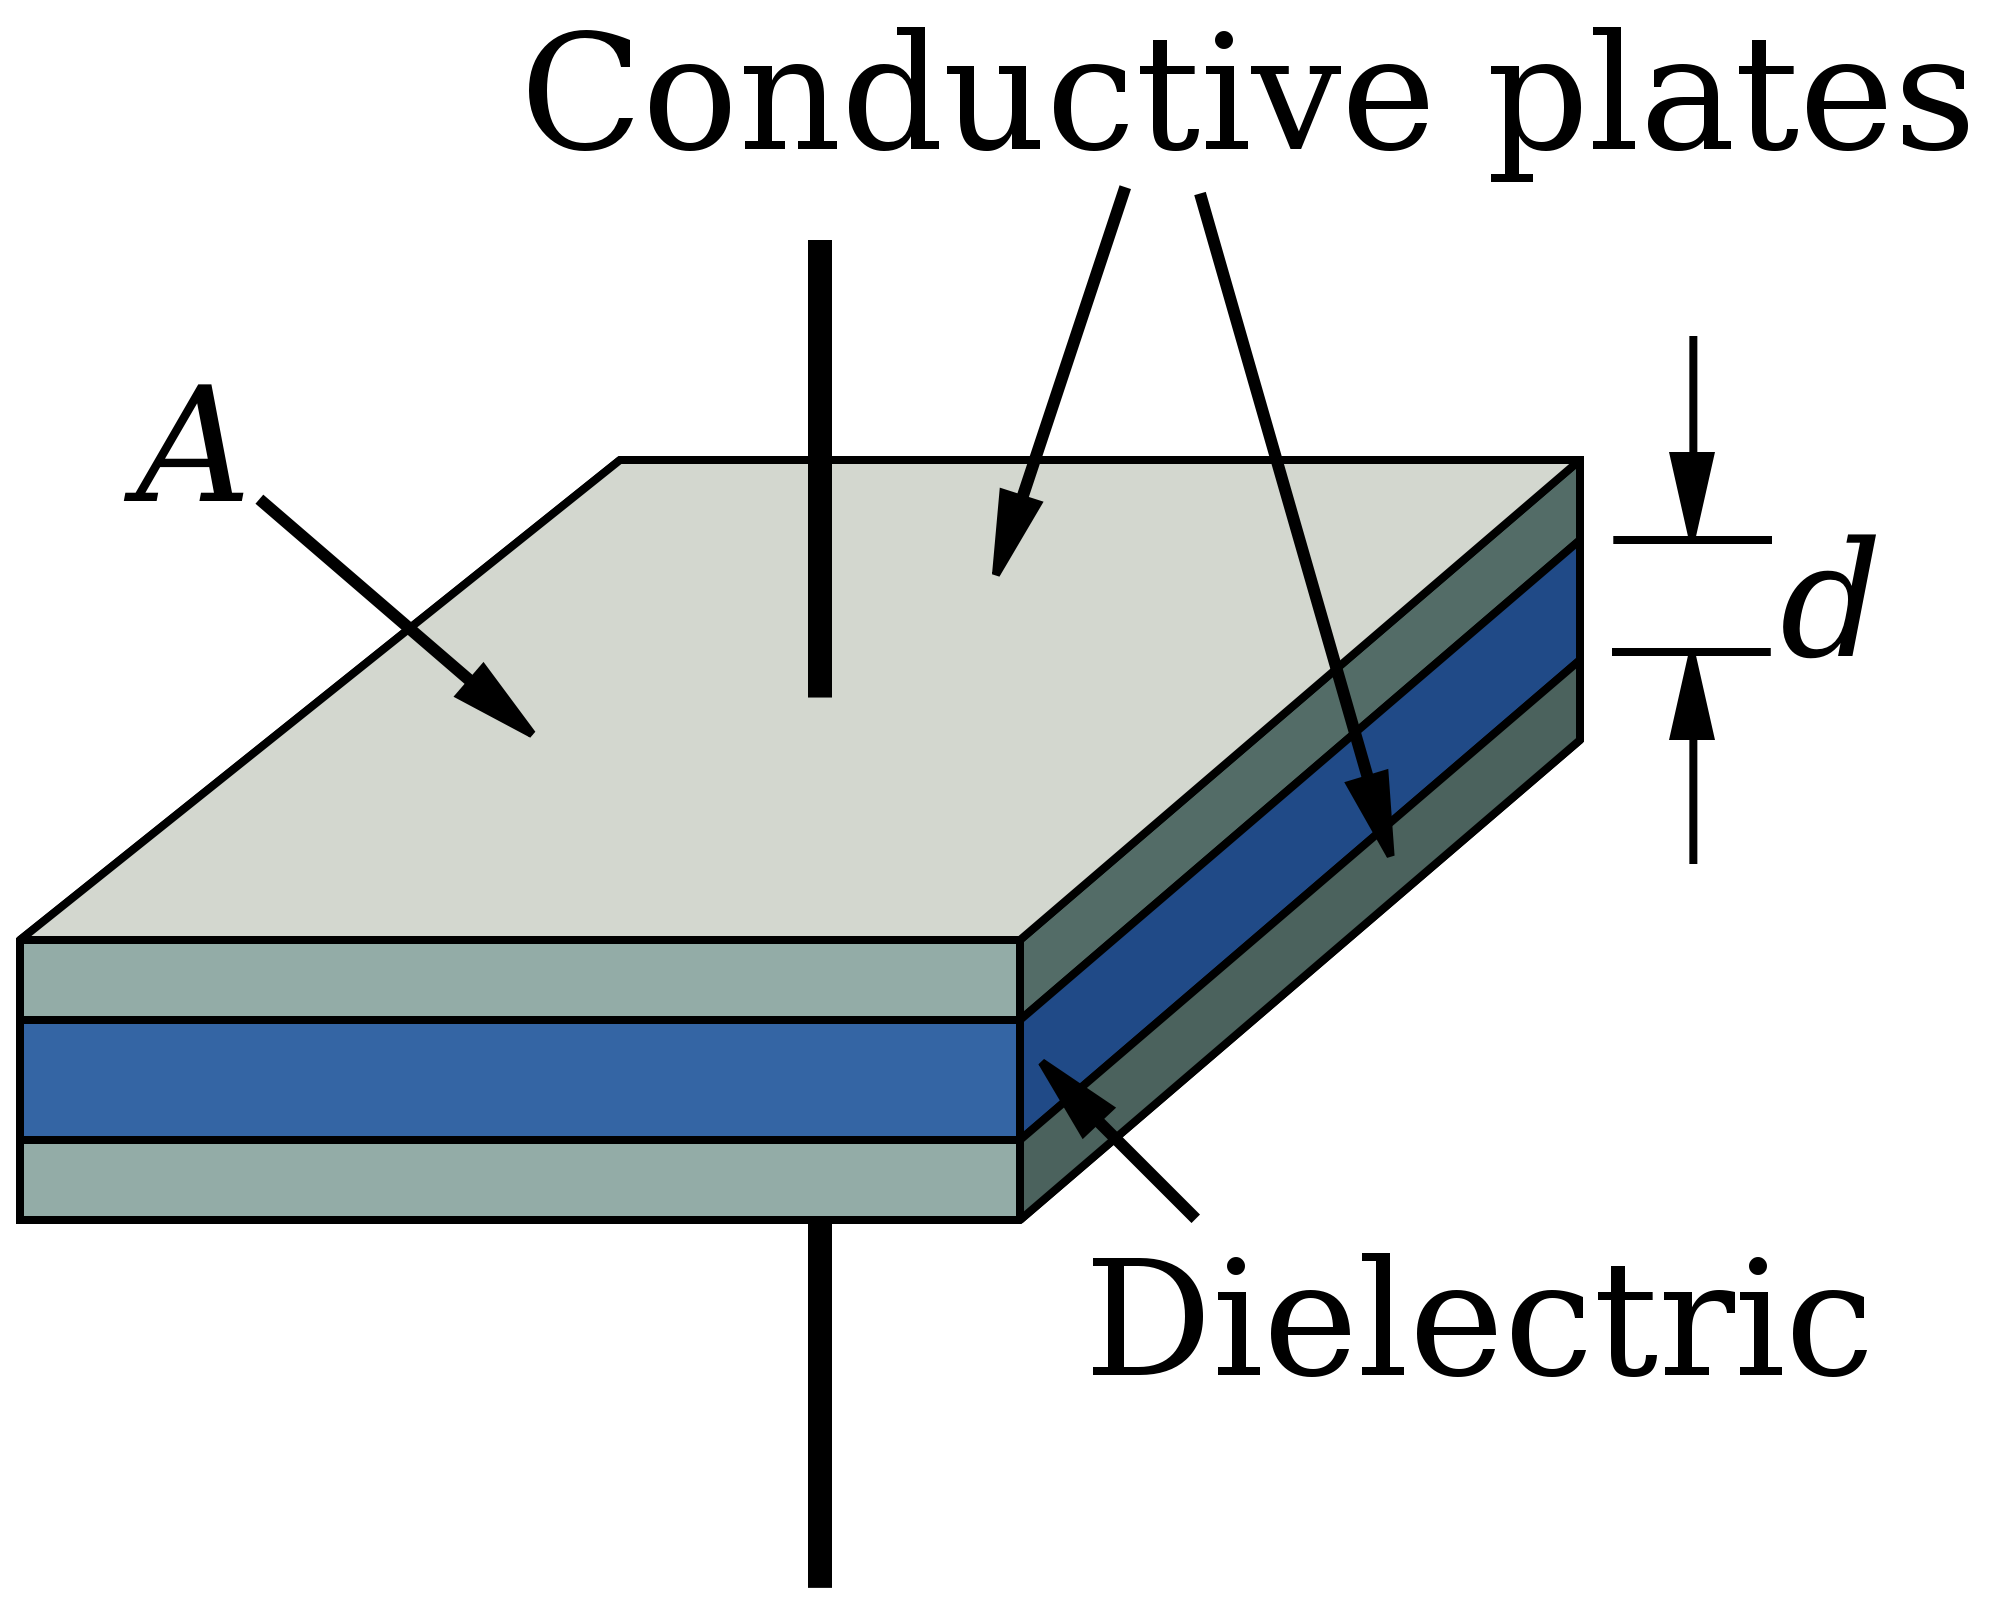
\includegraphics[width=0.4\textwidth]{img/plate1.png}
				\label{fig:plate1}	
				}
			\quad
				\subfigure[Edge Effect]{
				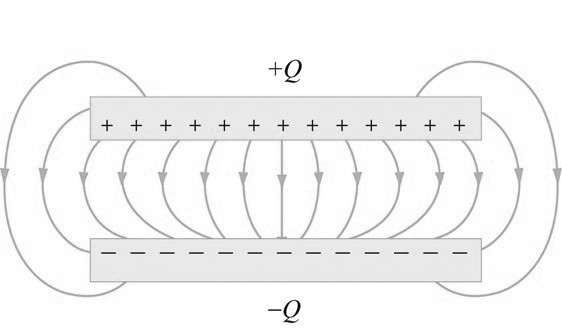
\includegraphics[width=0.4\textwidth]{img/edgeeff.jpg}
				\label{fig:edge}
				}
			\caption{Parallel Plate Capacitor and it's Edge Effect}
		\end{figure}
	
	무한히 넓은 이상적인 평행판 축전기의 전기력선은 평행하지만 유한한 크기의 평행판 축전기의 전기장은 Figure \ref{fig:edge}
	처럼 모서리에 가까워질수록 휘어진다. 이를 Edge Effect라고 한다. 그러나 A가 d에 비혜 충분히 크면 Edge Effect는 무시할 수 있을만큼 작아지므로 본 실험에서는 축전기의 전기장이 평행하다고 가정한다. 

\newpage
	본 실험에서는 전압과 축전기의 기하학적 구조를 바꿨을 때 축전기 극판 사이의 힘이 어떻게 변하는지 살펴보았다. 축전기에 걸린 전압을 $V$, 축전기의 간격을 $d$라고 했을 때 축전기의 사이의 전기장은 다음과 같다.
		\begin{equation} \label{eq:efd}
			E=\frac{V}{d}
		\end{equation}
	그런데 이 전기장은 두 극판이 만들어낸 전기장의 합이므로 한 쪽 극판이 받는 전기장은 (\ref{eq:efd})의 절반인 $E=V/{2d}$이다.

	극판이 받는 힘은 $F=QE$이고 $Q=CV$이므로 식(\ref{eq:ppl})을 대입하면 다음을 얻는다. 
		\begin{equation} \label{eq:force}
			F=\frac{\epsilon{}AV^{2}}{2d^{2}}
		\end{equation}


	축전기는 회로 요소이므로 병렬연결, 직렬연결에 대한 합성 전기용량을 구할 수 있다.
	축전기가 병렬연결되어있을 경우 양 극판에 걸린 전압의 크기가 $V$로 같고 총 전하량은 $Q=Q_1+Q_2$이므로 식(\ref{eq:qcv})을 대입하면 다음을 얻는다. 
		\begin{equation}
			CV=Q=Q_{1}+Q_{2}=C_{1}V+C_{2}V=(C_{1}+C_{2})V 
		\end{equation}

	이를 정리하면 다음과 같다.
		\begin{equation}
			C=C_{1}+C_{2}
		\end{equation}
	
	축전기가 직렬연결되어있을 경우 두 극판에 축적된 전하의 크기가 같고 총 전압은 $V=V_1+V_2$이므로 식(\ref{eq:qcv})을 대입하면 다음을 얻는다.
		\begin{equation}
			\frac{Q}{C}=V=V_{1}+V_{2}=\frac{Q}{C_1}+\frac{Q}{C_2}
		\end{equation}

	이를 정리하면 다음과 같다.
		\begin{equation}
			\frac{1}{C}=\frac{1}{C_1}+\frac{1}{C_2}
		\end{equation} 


	본 실험에서는 위의 식들을 이용하여 조건이 바뀌었을 때 두 극판 사이의 힘이 어떤 식으로 작용하는 지 알아본다. 

\newpage
\section{Method}
	\begin{figure}[h]
		\centering
		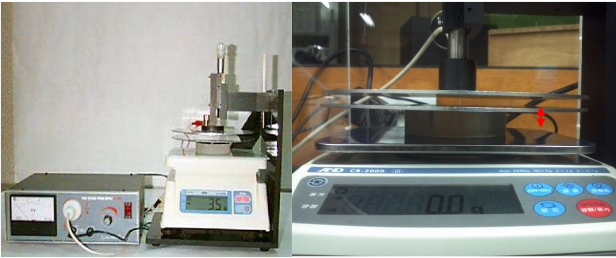
\includegraphics[width=0.7\textwidth]{img/expconfig.png}
		\caption{실험 장치}
	\end{figure}
	\noindent준비물: 전원, 저울, 전압계, 평행판 축전기, 평행판 거리 조절기, 1.35cm 유리판, 1.35cm 아크릴판\\
	\indent극판이 받는 힘이 바뀌면 극판이 저울에 가하는 수직항력이 바뀌므로 저울 값의 변화로부터 극판이 받는 힘의 변화를 측정할 수 있다. 따라서 거리 조절기로 극판 사이의 거리, 전원의 전압, 유전체의 유전율을 조절하면서 저울의 값을 기록하면 극판이 받는 힘의 변화와 앞선 물리량의 관계에 대해 알 수 있다.\\
	평행판의 반지름은 10\si{cm}으로 측정되었다.

\subsection{거리에 따른 전기력의 변화}
	전원의 전압을 5\si{kV}로 놓고 두 극판 사이에는 아무 것도 넣지 않았다($\epsilon{}_{air} \approx 1$).
	이 때 극판 사이의 거리 $d$를 각각 1.3, 1.2, 1.1, 1.0, 0.9, 0.8, 0.7\si{cm}로 놓고 전원 장치를 킨 후 저울에 나타난 숫자를 측정하였다.

\subsection{전압에 따른 전기력의 변화}
	극판 거리를 1\si{cm}로 놓고 두 극판 사이에는 아무 것도 넣지 않았다($\epsilon{}_{air} \approx 1$).
	이 때 전원의 전압 $V$를 각각 0, 1.5, 3, 4.5, 6, 7,5, 9\si{kV}로 놓고 전원 장치를 킨 후 저울에 나타난 숫자를 측정하였다. 
	전압의 간격을 1.5\si{kV}로 설정한 것은 1.5\si{kV}가 저울의 눈금변화가 나타난 최소 전압이었기 때문이다.

\subsection{유전율에 따른 전기력의 변화}
	극판 사이에 1.35\si{cm} 유리와 아크릴을 끼워넣었다. 1.35\si{cm}는 유리와 아크릴을 넣고 조였을 때의 간격이다.
	전압을 유리에서는 1\si{kV}, 아크릴에서는 2.5, 5\si{kV}로 설정했다. 
	유리에서는 1\si{kV}이상에서 장비에서 고주파음이 들려서 고주파음이 들리지 않는 최대치로 설정한 것이다. 
	그 이하에서는 저울의 눈금변화가 없어서 실험하지 못했다. 
	아크릴에서도 고주파음이 들리지 않는 최대치와 그 절반값을 실험대상으로 삼았다.  

\newpage

\section{Result}

\newpage

\section{Conclusion}
	
\section{Reference}

\end{document} 

%실험에서 개선할 점 등 피피티에서 봤던 거 모두 적어서 처리합시다.
